\section{Questões}\label{sec:questoes}


\subsection{Questão 1}
Indique as etapas, como na Tabela 3.14, do algoritmo de busca direta à medida que ele monta o
banco de dados de roteamento para o nó A na rede mostrada na Figura 3.59.

\begin{figure}[H]
    \centering
    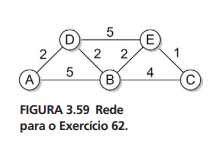
\includegraphics[width=0.7\textwidth]{images/ex_62.png}
    \caption{Rede mostrada na questão 1}
    \label{fig:questao_1}
\end{figure}

\begin{figure}[H]
    \centering
    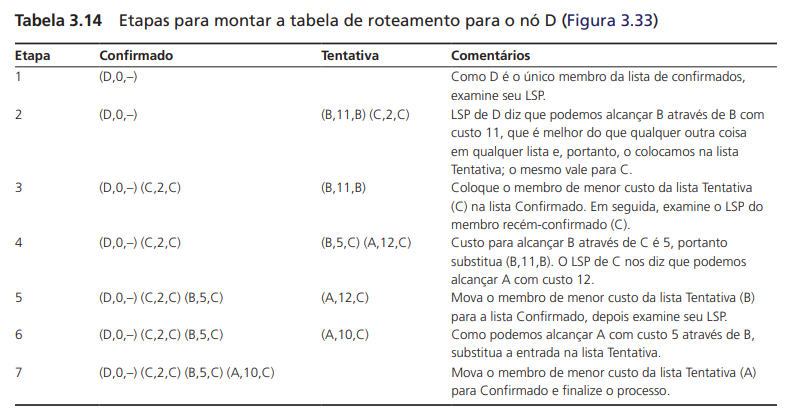
\includegraphics[width=0.9\textwidth]{images/tabela_3_14.png}
    \caption{Tabela 3.14 usada como referência para a questão} 
    \label{fig:questao_1_tabela}
\end{figure}

\textbf{Resposta:} \\
A seguir, apresentamos as etapas do algoritmo de estado de enlace (Dijkstra) aplicadas ao nó A. O procedimento é análogo ao apresentado na Tabela 3.14 da obra de Peterson e Davie, considerando as informações de custo da Figura 3.59.

\begin{table}[h!]
\centering
\resizebox{\textwidth}{!}{
\begin{tabular}{|c|l|l|p{8.8cm}|}
\hline
\textbf{Etapa} & \textbf{Confirmado} & \textbf{Tentativa} & \textbf{Comentários} \\ \hline
1 & (A,--,--) & (D,2,A), (B,5,A) & LSP de A indica vizinhos D (custo 2) e B (custo 5). \\ \hline
2 & (A,--,--), (D,2,A) & (B,5,A), (E,7,D) & D é o nó de menor custo. Através de D, E é alcançável com custo total 7 (2+5). \\ \hline
3 & (A,--,--), (D,2,A), (B,5,A) & (E,7,D), (C,9,B) & B tem menor custo. B conecta-se a C com custo adicional de 4, totalizando 9. \\ \hline
4 & (A,--,--), (D,2,A), (B,5,A), (E,7,D) & (C,8,E) & E tem menor custo. E conecta-se a C com custo adicional de 1, totalizando 8. Melhor que custo anterior. \\ \hline
5 & (A,--,--), (D,2,A), (B,5,A), (E,7,D), (C,8,E) & -- & C é o último nó. Tabela de roteamento finalizada. \\ \hline
\end{tabular}
}
\caption{Etapas do algoritmo de busca direta (Dijkstra) para o nó A.}
\end{table}


\vspace{0.5cm}
\textbf{Resumo das rotas a partir de A:}

\begin{itemize}
    \item Para D: custo 2, próximo salto: D
    \item Para B: custo 5, próximo salto: B
    \item Para E: custo 7, próximo salto: D
    \item Para C: custo 8, próximo salto: E
\end{itemize}

\vspace{0.5cm}
\textbf{Fonte:} Peterson, L. L., \& Davie, B. S. \textit{Redes de Computadores - Uma abordagem top-down}, Elsevier. Figura 3.59 e Tabela 3.14.

\subsection{Questão 2}
Suponha que um roteador tenha montado a tabela de roteamento mostrada na Tabela 3.18. O
roteador pode entregar pacotes diretamente pelas interfaces 0 e 1, ou então pode encaminhar
pacotes aos roteadores R2, R3 ou R4. Descreva o que o roteador faz com um pacote endereçado a
cada um dos seguintes destinos:

\begin{enumerate}[label=\alph*.]
    \item 128.96.39.10
    \item 128.96.40.12
    \item 128.96.40.151
    \item 192.4.153.17
    \item 192.4.153.90
\end{enumerate}

\begin{figure}[H]
    \centering
    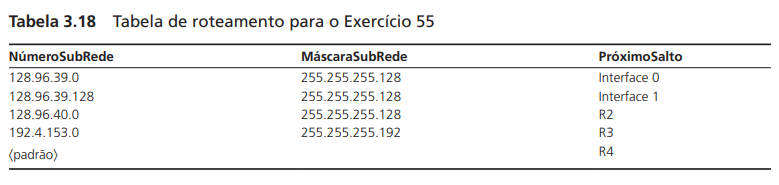
\includegraphics[width=0.9\textwidth]{images/tabela_3_18.png}
    \caption{Tabela 3.18 usada como referência para a questão} 
    \label{fig:questao_2_tabela}
\end{figure}

\textbf{Resposta:}
\begin{enumerate}[label=\textbf{\alph*}.]
    \item \textbf{128.96.39.10} \\
    A sub-rede \texttt{128.96.39.0} com máscara \texttt{255.255.255.128} cobre o intervalo de endereços de \texttt{128.96.39.0} até \texttt{128.96.39.127}. Como o endereço de destino está nesse intervalo, o pacote é encaminhado pela \textbf{Interface 0}.
    
    \item \textbf{128.96.40.12} \\
    A sub-rede \texttt{128.96.40.0} com máscara \texttt{255.255.255.128} cobre o intervalo de \texttt{128.96.40.0} até \texttt{128.96.40.127}. O endereço \texttt{128.96.40.12} está contido nesse intervalo, portanto o pacote será encaminhado ao \textbf{roteador R2}.
    
    \item \textbf{128.96.40.151} \\
    Esse endereço não é coberto por nenhuma das sub-redes específicas na tabela. Portanto, aplica-se a rota padrão. O pacote será encaminhado para o \textbf{roteador R4}.
    
    \item \textbf{192.4.153.17} \\
    A sub-rede \texttt{192.4.153.0} com máscara \texttt{255.255.255.192} cobre o intervalo de \texttt{192.4.153.0} até \texttt{192.4.153.63}. Como \texttt{192.4.153.17} está nesse intervalo, o pacote será encaminhado para o \textbf{roteador R3}.
    
    \item \textbf{192.4.153.90} \\
    Esse endereço está fora do intervalo da sub-rede \texttt{192.4.153.0/26}, e não há outra entrada correspondente. Portanto, o pacote será enviado para o \textbf{roteador R4} (rota padrão).
\end{enumerate}

\textbf{Fonte:} Peterson, L. L., \& Davie, B. S. \textit{Redes de Computadores - Uma abordagem top-down}, Elsevier. Tabela 3.18.

\subsection{Questão 3}
A Tabela 3.20 é uma tabela de roteamento usando CIDR. Os bytes de endereço estão em
hexadecimal. A notação “/12” em C4.50.0.0/12 indica uma máscara de rede com 12 bits 1 iniciais:
FF.F0.0.0. Observe que as três últimas entradas abrangem cada endereço e, portanto, podem ser usadas no lugar de uma rota padrão. 
Indique para qual próximo salto os pacotes com os seguintes endereços serão entregues:

\begin{enumerate}[label=\alph*.]
    \item C4.5E.13.87
    \item C4.5E.22.09
    \item C3.41.80.02
    \item 5E.43.91.12
    \item C4.6D.31.2E
    \item C4.6B.31.2E
\end{enumerate}

\begin{figure}[H]
    \centering
    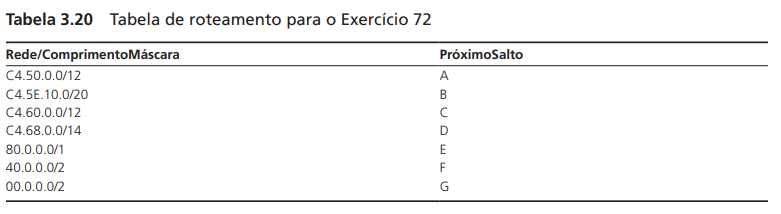
\includegraphics[width=0.9\textwidth]{images/tabela_3_20.png}
    \caption{Tabela 3.20 usada como referência para a questão} 
    \label{fig:questao_3_tabela}
\end{figure}

\textbf{Resposta:}
Para cada escolher cada salto, basta escolher o endereço mais específico, ou seja, o que
possui a maior quantidade de bits 1 na máscara.\\

\begin{table}[ht]
\centering
\caption{Associação de endereços aos prefixos CIDR e próximos saltos}
\label{tab:roteamento}
\begin{tabular}{llll}
\toprule
\textbf{Endereço}      & \textbf{Prefixo que casa} & \textbf{Máscara} & \textbf{Próx.\ Salto} \\
\midrule
C4.5E.13.87 & C4.5E.10.0  & /20 & B \\
C4.5E.22.09 & C4.50.0.0   & /12 & A \\
C3.41.80.02 & 80.0.0.0    & /1  & E \\
5E.43.91.12 & 40.0.0.0    & /2  & F \\
C4.6D.31.2E & C4.60.0.0   & /12 & C \\
C4.6B.31.2E & C4.68.0.0   & /14 & D \\
\bottomrule
\end{tabular}
\end{table}
\FloatBarrier

\textbf{Fonte:} Peterson, L. L., \& Davie, B. S. \textit{Redes de Computadores - Uma abordagem top-down}, Elsevier. Tabela 3.20.

\subsection{Questão 4}
Leiam a Seção 4.2 do livro-texto (exceto os trechos sobre “Multicast
interdomínios - MSDP” e “Árvores bidirecionais - BIDIR-PIM”) e respondam:

\begin{enumerate}[label=\alph*.]
    \item Além da entrega de pacotes aos destinos, qual é a principal preocupação de um
    protocolo de roteamento multicast?
    \item Qual é o papel do IGMP no esquema de funcionamento multicast do IP?
    \item Compare brevemente as estratégias DVMRP e PIM-SM, mostrando as vantagens e
    desvantagens de cada uma.
    \item Que características adicionais o PIM-SSM traz em relação ao PIM-SM?
\end{enumerate}

\textbf{Resposta:}
\begin{enumerate}[label=\alph*.]
    \item A prevenção de loops de roteamento é a principal preocupação, garantindo que pacotes não sejam replicados indefinidamente. Para isso, os protocolos multicast utilizam:\\
Verificação RPF (Reverse Path Forwarding): Confere se a interface de entrada do pacote é a mesma usada para rotas unicast até a origem, descartando pacotes com caminhos inválidos.\\
Escopo administrativo: Limita o alcance de endereços multicast específicos para evitar vazamentos entre domínios.\\
Árvores de distribuição: Construídas com base no caminho mais curto (SPT) ou em árvores compartilhadas (RP), minimizando replicações desnecessárias\\

\item Papel do IGMP no multicast IP
O IGMP (Internet Group Management Protocol) gerencia a associação de hosts a grupos multicast:

Ingresso em grupos: Hosts enviam mensagens Membership Report para solicitar entrada em um grupo (endereço 224.0.0.0/4).

Consulta periódica: Roteadores enviam Membership Query para verificar interesse contínuo dos hosts.

Controle de saída: Em IGMPv2+, hosts podem enviar Leave Group para sair de um grupo, otimizando o uso de largura de banda.

Filtragem de fontes: IGMPv3 permite que hosts especifiquem quais origens aceitam (ex: permitir apenas tráfego de S1 para o grupo G)

\item Comparação entre DVMRP e PIM-SM
\begin{table}[ht]
\centering
\caption{Comparação entre DVMRP e PIM-SM}
\label{tab:multicast}
\begin{tabular}{|l|p{6cm}|p{6cm}|}
\hline
\textbf{Critério} & \textbf{DVMRP} & \textbf{PIM-SM} \\ 
\hline
Estratégia & Modo denso (flood-and-prune) & Modo esparso (junção explícita via RP) \\
\hline
Eficiência & Ideal para redes densas, mas ineficiente em redes esparsas & Reduz inundação usando RP como ponto central \\
\hline
Complexidade & Mantém tabela de roteamento própria & Usa tabela unicast existente \\
\hline
Escalabilidade & Limitada (alto overhead de controle) & Superior (adequado para redes grandes) \\
\hline
Flexibilidade & Suporta apenas árvores (S,G) & Permite transição entre (*,G) e (S,G) \\
\hline
Vantagens & - & Menor consumo de banda em redes esparsas, independência do protocolo unicast \\
\hline
Desvantagens & Gera tráfego excessivo em redes esparsas & Dependência inicial do RP \\
\hline
\end{tabular}
\end{table}
\newpage

\textbf{Vantagens do PIM-SM:}

Menor consumo de largura de banda em redes esparsas.

Independência do protocolo unicast subjacente.

\textbf{Desvantagens do DVMRP:}

Gera tráfego excessivo em redes esparsas.

Não escala bem para redes complexas

\item O PIM-SSM (Source-Specific Multicast) introduz melhorias em relação ao PIM-SM:

Eliminação do RP: Conexões são estabelecidas diretamente entre receptores e fontes usando pares (S,G), removendo a dependência de um ponto único de falha.

Segurança reforçada: Receptores especificam explicitamente a fonte permitida, impedindo ataques com tráfego de origens não autorizadas.

Redução de overhead: Não requer mensagens de registro ou descoberta de fontes (MSDP).

Adequação a aplicações 1:N: Ideal para transmissão de TV/IP ou streaming, onde há uma única fonte para múltiplos receptores.

Exemplo: Em um serviço de streaming, um cliente solicita o canal (S=192.0.2.10, G=232.1.1.1). O roteador encaminha o tráfego apenas dessa fonte, ignorando outras
\end{enumerate}

\textbf{Fonte:} Peterson, L. L., \& Davie, B. S. \textit{Redes de Computadores - Uma abordagem top-down}, Elsevier, Seção 4.2 (págs. 221-231).